\section{Multilayer Perceptron}

\subsection{Methods}

\subsubsection{Treatment of Data}

\paragraph{Splitting}

\paragraph{Preprocessing}
Preprocessing consisted of normalizing the data.

\subsubsection{MLP setup}

\begin{figure}
	\centering
	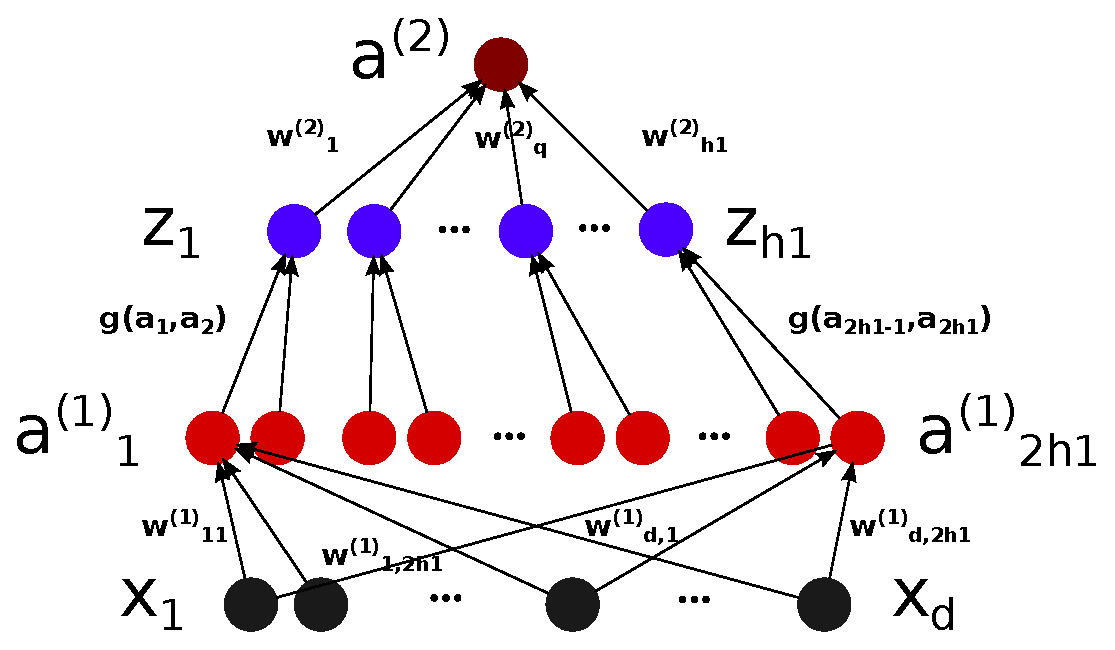
\includegraphics[width=.8\textwidth]{mlp/mlp.eps}
	\label{mlp}
	\caption{dfdf}
\end{figure}

\paragraph{Early stopping}
Evaluate empirical error $\hat{R}(\hat{f};\mathcal{D}_V)$ for validation set $\mathcal{D}_V$ along-side the training-error $\hat{R}(\hat{f};\mathcal{D}_T)$while training the MLP on $\mathcal{D}_T$. Stop at the training at the epoch where the validation error stops decreasing and starts increasing. 
\subsubsection{Parameters for subtasks}

\subsubsection{Examples of overfitting}

\section{Results}